
\documentclass[11 pt,t]{beamer}
\usepackage{verbatim}
\usepackage{latexsym}
\usepackage{amsfonts,amssymb}
\graphicspath{{figures/}}    
\usetheme[
	bullet=circle,		% Other option: square
	bigpagenumber,		% circled page number on lower right
	topline=true,		% colored bar at the top of the frame 
	]{Zurich}

\tikzstyle{decision} = [diamond, draw, fill=blue!20,
text width=4.5em, text badly centered, node distance=3cm, inner sep=0pt]
\tikzstyle{block} = [rectangle, draw, fill=blue!20,
text width=5em, text centered, rounded corners, minimum height=4em]
\tikzstyle{line} = [draw, -latex']
\tikzstyle{cloud} = [draw, ellipse,fill=red!20, node distance=3cm,
    minimum height=2em]
\usetikzlibrary{arrows}
\usetikzlibrary{decorations.pathreplacing}
\makeatletter
% add a macro that saves its argument
\newcommand{\footlineextra}[1]{\gdef\insertfootlineextra{#1}}
\newbox\footlineextrabox
 
% add a beamer template that sets the saved argument in a box.
% The * means that the beamer font and color "footline extra" are automatically added. 
\defbeamertemplate*{footline extra}{default}{
  \begin{beamercolorbox}[ht=2.25ex,dp=1ex,leftskip=\Gm@lmargin]{footline extra}
    \insertfootlineextra
    % \par\vspace{2.5pt}
  \end{beamercolorbox}
}
 
\addtobeamertemplate{footline}{%
  % set the box with the extra footline material but make it add no vertical space
  \setbox\footlineextrabox=\vbox{\usebeamertemplate*{footline extra}}
  \vskip -\ht\footlineextrabox
  \vskip -\dp\footlineextrabox
  \box\footlineextrabox%
}
{}
 
% patch \begin{frame} to reset the footline extra material
\let\beamer@original@frame=\frame
\def\frame{\gdef\insertfootlineextra{}\beamer@original@frame}
\footlineextra{}
\makeatother
%-----------------------------------------------------------------------------
% DOCUMENT PROPERTIES
\logo{\includegraphics[scale=0.13]{ouclogo.png}}
\author{DingHao}
\title{Multi-class Imbalanced Learning}

%-----------------------------------------------------------------------------


\begin{document}


% ----------------------------------------------------------------------------
\frame{\titlepage}
\frame{\frametitle{Contents}\tableofcontents}
% ----------------------------------------------------------------------------


\section{Introduction}

\begin{frame}
\frametitle{Introduction}
\framesubtitle{Classification Problem}
\begin{minipage}[t]{\linewidth}\centering
\begin{figure}
   \includegraphics[width=10cm]{clean}

\end{figure}
\end{minipage}
\end{frame}

\begin{frame}
\frametitle{Introduction}
\framesubtitle{classifiers}
\begin{minipage}[t]{\linewidth}\centering
\begin{figure}
   \includegraphics[width=10cm]{1}
\end{figure}
\end{minipage}
\end{frame}

\begin{frame}
\frametitle{Introduction}
\framesubtitle{classifiers}
\begin{minipage}[t]{\linewidth}\centering
\begin{figure}
   \includegraphics[width=10cm]{2}
\end{figure}
\end{minipage}
\end{frame}

\begin{frame}
\frametitle{Introduction}
\framesubtitle{classifiers}
\begin{minipage}[t]{\linewidth}\centering
\begin{figure}
   \includegraphics[width=10cm]{3}
\end{figure}
\end{minipage}
\end{frame}

\begin{frame}
\frametitle{Introduction}
\framesubtitle{Real World}
\begin{minipage}[t]{\linewidth}\centering
\begin{figure}
   \includegraphics[width=10cm]{messy}
\end{figure}
\end{minipage}
\end{frame}


\begin{frame}
\frametitle{Introduction}
\framesubtitle{Doggy}
\begin{minipage}[t]{\linewidth}\centering
\begin{figure}
   \includegraphics[width=8cm]{dog}
\end{figure}
\end{minipage}
\end{frame}

\begin{frame}
\frametitle{Introduction}
\framesubtitle{Rare Word}
\begin{minipage}[t]{\linewidth}\centering
\begin{figure}
   \includegraphics[width=8cm]{shengpizi}
\end{figure}
\end{minipage}
\end{frame}

\begin{frame}
\frametitle{Introduction}
\framesubtitle{Rare Word}
\begin{minipage}[t]{\linewidth}\centering
\begin{figure}
   \includegraphics[width=8cm]{shengpizi1}
\end{figure}
\end{minipage}
\end{frame}

\begin{frame}
\frametitle{Introduction}
\framesubtitle{Imbalanced Ratio}
imbalanced ratio = majority class / minority class
\begin{block}{ZooScan}
   427 / 28 = 15.25
\end{block}
\begin{exampleblock}{Kaggle}
   1979 / 9 = 219.89
\end{exampleblock}
\begin{alertblock}{WHOI}
   2606720 / 4 = 651680
\end{alertblock}
{\textcolor{tangocolordarkchameleon}{EVEN MORE THAN $10^{8}$ !} }
\end{frame}

\begin{frame}
\frametitle{Introduction}
\begin{center}%\begin{minipage}[t]{\linewidth}\centering

\Huge{WHY?}

%\end{minipage}
\end{center}
\end{frame}
% ----------------------------------------------------------------------------

\section{Evaluation Criteria}
\begin{frame}
\frametitle{Evaluation Criteria}

\begin{minipage}[t]{\linewidth}\centering
\begin{figure}
   \includegraphics[width=7cm]{rate}
\end{figure}
\end{minipage}
\begin{displaymath}
G-mean = \sqrt{TPr * TNr}
\end{displaymath}
\begin{displaymath}
Precision = \frac{TP}{TP+FP}
\end{displaymath}
\begin{displaymath}
Recall = \frac{TP}{TP+FN} = TPr
\end{displaymath}
\begin{displaymath}
F-measure = \frac{2*Precision*Recall}{Precision+Recall}
\end{displaymath}
\end{frame}

% ----------------------------------------------------------------------------
\section{Approaches}
\begin{frame}
\frametitle{Approaches}
\framesubtitle{Overview}
\begin{itemize}
\item Sampling\\
\emph{Under-sampling}\\
\emph{Over-samping}
\item Cost-sensitive learning
\item Ensembled classifier\\
\emph{EasyEnsemble}\\
\emph{BalanceCascade}
\end{itemize}
\end{frame}

\begin{frame}
\frametitle{Approaches}
\framesubtitle{Sampling}
\begin{minipage}[t]{\linewidth}\centering
\begin{figure}
   \includegraphics[width=6cm]{sampling}
\end{figure}
\end{minipage}
{\textcolor{tangocolordarkscarletred}{Best approache: SMOTE}}
\end{frame}

\begin{frame}
\frametitle{Approaches}
\framesubtitle{Cost-sensitive}
\begin{displaymath}
L(x,i) = \sum_{j}P(j|x)c(i,j)
\end{displaymath}
Minimize the overall cost.
\begin{itemize}
\item[-] x : an example
\item[-] i : a class
\item[-] j : the j$^{th}$ class
\item[-] P : Probability
\item[-] c : cost matrix
\end{itemize}
{\textcolor{tangocolordarkscarletred}{Best approaches: AdaCost, AsymBoost}}
\end{frame}

\begin{frame}
\frametitle{Approaches}
\framesubtitle{Ensembled Classifier}

\begin{center}
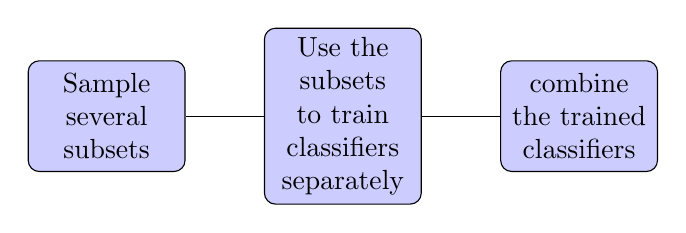
\begin{tikzpicture}[scale=0.7, node distance = 3.0cm, auto]
\node [block] (problem) {Sample several subsets};
\node [block, right of=problem] (model) {Use the subsets to train classifiers separately};
\path [block] (problem) -- (model);
\node [block, right of=model] (method) {combine the trained classifiers};
\path [block] (model) -- (method);
\end{tikzpicture}\\
\end{center}
{\textcolor{tangocolordarkscarletred}{Best approaches: EasyEnsemble, BalanceCascade, SMOTEBoost}}
\end{frame}

\begin{frame}
\frametitle{Approaches}
\framesubtitle{EasyEnsemble.M $\Rightarrow$ EasyEnsemble.D}
\begin{table}[!ht]
%\centering
\toprule
\begin{tabular}{l p{.88\linewidth}}
\midrule
1:&Input:A set of minority class examples $\mathcal{P}$, k-1 sets of majority class examples $\mathcal{N}, |\mathcal{P}|<|\mathcal{N}_{k}|$, the number of subsets T to sample from $\mathcal{N}_{k}$, and $s_{i}$,the number of iterations to train an AdaBoost ensemble $H_{i}$\\
2:&for i$\Leftarrow$ 1:T\\ 
3:&\qquad$D_{i}=\mathcal{N}_{1}$\\
4:&\qquad for t$\Leftarrow$ 1:k\\ 
5:&\qquad \qquad Randomly sample a subset $\mathcal{N}_{it}$ from $\mathcal{N}_{k}$, $N_{it}$,$|N_{it}|=$\\&\qquad \qquad$|P|+\frac{\mathcal{N}_{1}*\left(|\mathcal{N}_{i}|-|P|\right)}{|\mathcal{N}_{k}|}$ in the $t^{th}$\\
6:&\qquad \qquad $D_{i}=D_{i}\bigcup\mathcal{N}_{it}$\\
7:&\qquad$H_{t}\left(x\right)=sgn\left(\sum^{s_{i}}_{d=1}\alpha _{t,d}h_{t,d}\left(x\right)-\theta_{i}\right)$\\
8:&$H\left(x\right)=sgn\left(\sum^{T}_{t=1}\sum^{s_{i}}_{d=1}\alpha _{t,d}h_{t,d}\left(x\right)-\sum^{T}_{t=1}\theta_{i}\right)$\\

\end{tabular}
\end{table}
\footlineextra{Q.-Q.Li, and X.-Y.Liu. ”EasyEnsemble.M for multiclass imbalance
problem.” In: Pattern Recognition and Artificial Intelligence
27.2(2014):187-192.}
\end{frame}

% ----------------------------------------------------------------------------

\section{Future Work}
\begin{frame}
\frametitle{Future Work}
\begin{itemize}
\item Optimize the algorithm to cost less runtime
\item Use Kaggle and WHOI datasets
\item Increase the amount of time in each dataset
\end{itemize}

\end{frame}

% ----------------------------------------------------------------------------
\usebackgroundtemplate{
   \includegraphics[width=\paperwidth,
                    height=\paperheight]{background}
}
\begin{frame}
\ \\ \ \\
\centering \Large \textcolor{white}{Q\&A}

\end{frame}
\usebackgroundtemplate{}
% ----------------------------------------------------------------------------


\end{document}
